  
%!TEX root = ../proposal.tex

\providecommand{\lightred}{red!75}
\providecommand{\lightblue}{blue!75}
\providecommand{\lightgreen}{green!75}
\providecommand{\offset}{.1}

\centering
\scalebox{1}{
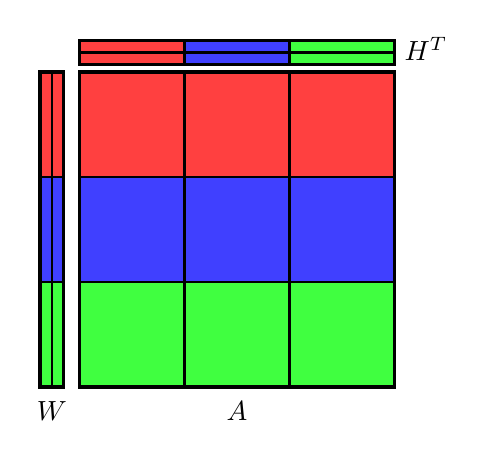
\begin{tikzpicture}

% draw A
\fill[\lightred] (0,8/3) rectangle ++(4,4/3);
\fill[\lightblue] (0,4/3) rectangle ++(4,4/3);
\fill[\lightgreen] (0,0) rectangle ++(4,4/3);
\node at (2,-3*\offset) {$\M{A}$};
\draw[thick,xscale=4/3,yscale=4/3] (0,0) grid ++(3,3);
\draw[very thick] (0,0) rectangle (4,4);

% draw W
\draw[fill=\lightred,shift={(-.5,0)}] (0,8/3) rectangle ++ (.3,4/3);
\draw[fill=\lightblue,shift={(-.5,0)}] (0,4/3) rectangle ++ (.3,4/3);
\draw[fill=\lightgreen,shift={(-.5,0)}] (0,0) rectangle ++ (.3,4/3);
\draw[thick,shift={(-.5,0)},xscale=.15,yscale=4/3] (0,0) grid ++(2,3);
\draw[very thick,shift={(-.5,0)}] (0,0) rectangle ++(0.3,4);
\node at (-.5+.15,-3*\offset) {$\M{W}$};

% draw H
\draw[fill=\lightred,shift={(0,4.1)}] (0,0) rectangle ++(4/3,.3);
\draw[fill=\lightblue,shift={(0,4.1)}] (4/3,0) rectangle ++(4/3,.3);
\draw[fill=\lightgreen,shift={(0,4.1)}] (8/3,0) rectangle ++(4/3,.3);
\draw[thick,shift={(0,4.1)},xscale=4/3,yscale=.15] (0,0) grid ++(3,2);
\draw[very thick,shift={(0,4.1)}] (0,0) rectangle ++(4,0.3);
\node at (4+4*\offset,4.3) {$\M{H}^T$};

\end{tikzpicture}
}